\subsection{Ozone mixing ratios as function of NOx and Temperature} \label{ss:r_contours}

\begin{figure}%
    \centering%
    \caption{Contours of maximum ozone mixing ratio as a function of the total \ce{NO_x} emissions on the first day and temperature for each chemical mechanism and using both a temperature-dependent and -independent source of isoprene emissions.}
    \label{f:ozone_contours}%
    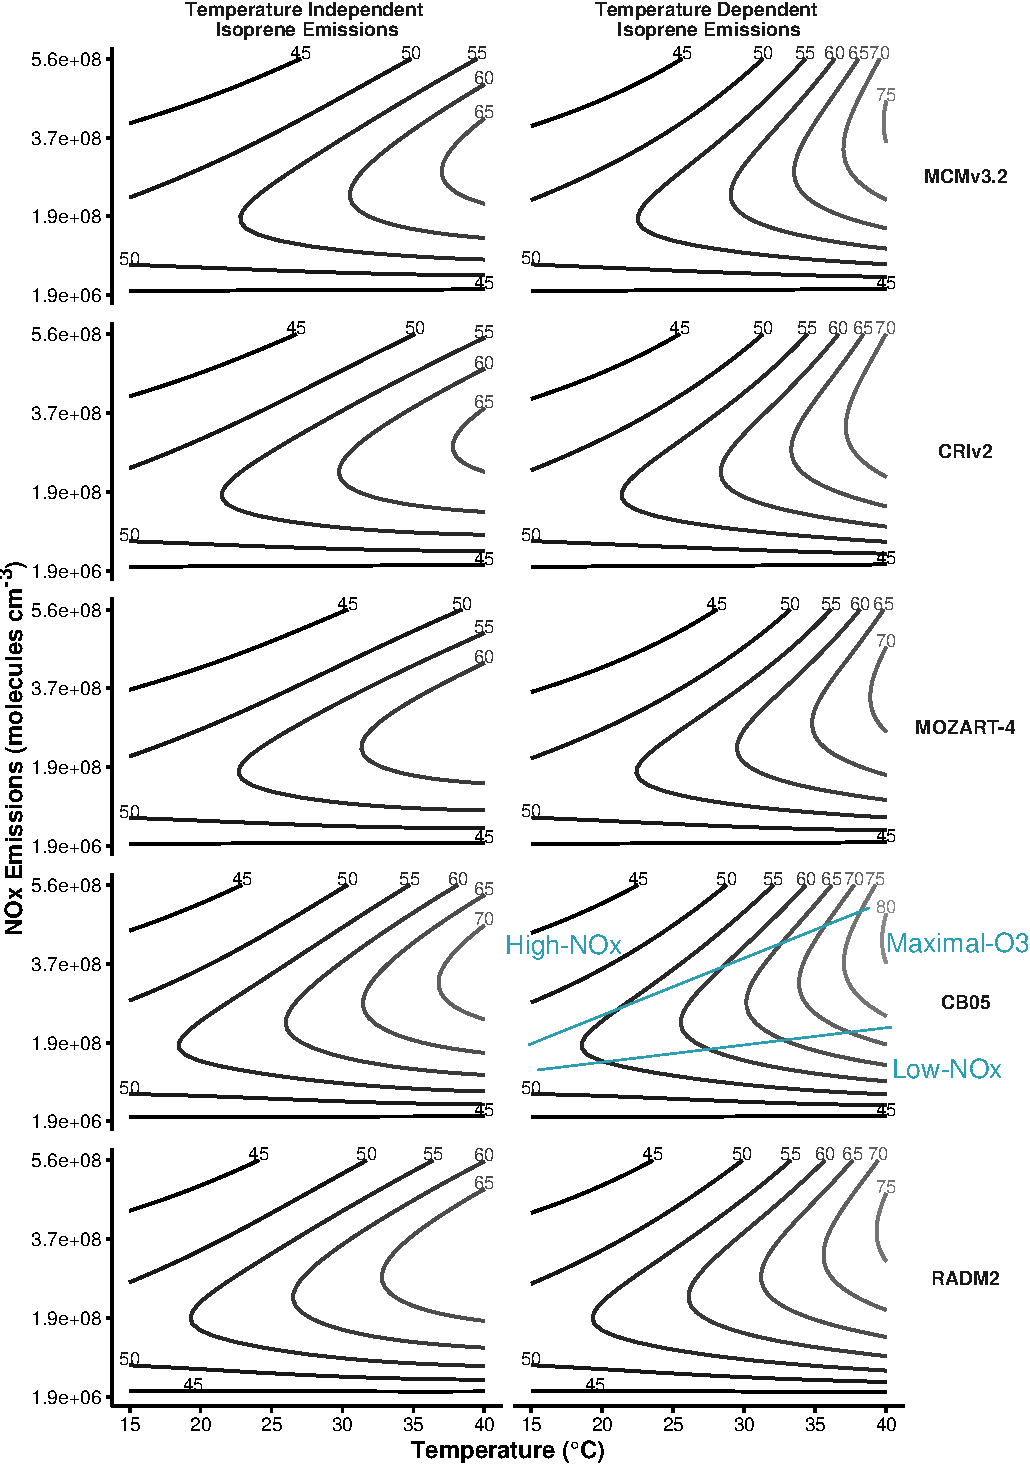
\includegraphics[width=\textwidth]{img/O3_comparison}%
\end{figure}

\begin{figure}[t]%
    \centering%
    \caption{Ozone mixing ratios at each temperature are allocated to different \ce{NO_x}-regimes of Fig.~\ref{f:ozone_contours}. The differences in ozone mixing ratios due to chemistry and emissions of Table~\ref{t:differences} are represented graphically for MOZART-4, the approach was used to calculate the differences with each chemical mechanism.}%
    \label{f:O3-T}%
    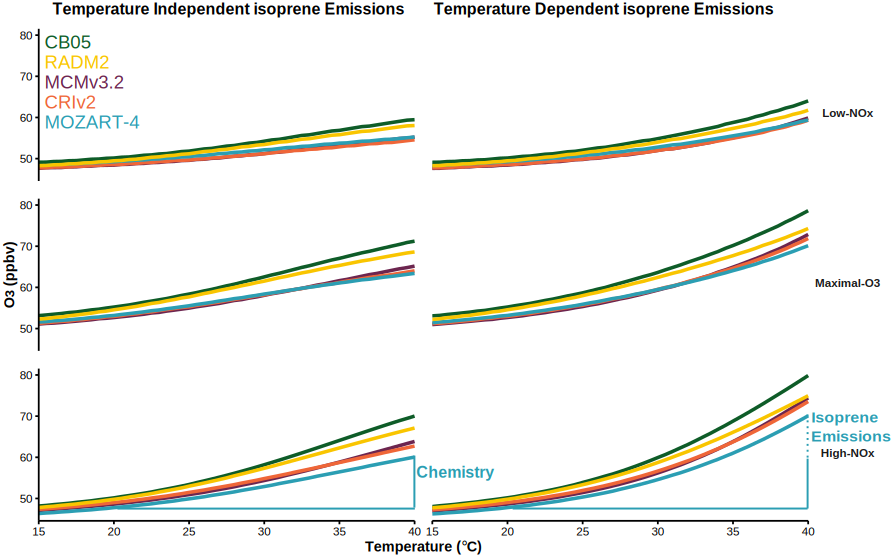
\includegraphics[width=\textwidth]{img/O3-T_correlation}%
\end{figure}

\begin{table}%
    \centering%
    \caption{Increase in ozone mixing ratio (ppbv) due to chemistry and emissions at $40$~\degree C from reference temperature ($20$~\degree C) in the \ce{NO_x}-regimes of Fig.~\ref{f:ozone_contours}.}%
    \label{t:differences}%
    \begin{tabularx}{\textwidth}{c|c *{3}{|c}} 
    \hline \hline
    \textbf{Chemical} & \textbf{Source of} & \multicolumn{3}{c}{\textbf{Increase in Ozone from 20~$^{\circ}$C to 40~$^{\circ}$C (ppbv)}} \\ \cline{3-5}
    \textbf{Mechanism} & \textbf{Difference} & \textbf{Low-\chem{NO_x}} & \textbf{Maximal-\chem{O_3}} & \textbf{High-\chem{NO_x}} \\ 
    \hline \hline
    \multirow{2}{*}{MCMv3.2} & Isoprene Emissions & 4.6 & 7.7 & 10.6 \\ 
    & Chemistry & 6.8 & 12.5 & 15.2 \\ \hline
    \multirow{2}{*}{CRIv2} & Isoprene Emissions & 4.8 & 7.9 & 10.8 \\
    & Chemistry & 6.0 & 11.1 & 13.7 \\ \hline
    \multirow{2}{*}{MOZART-4} & Isoprene Emissions & 4.1 & 6.7 & 10.0 \\
    & Chemistry & 6.0 & 10.2 & 12.3 \\ \hline
    \multirow{2}{*}{CB05} & Isoprene Emissions & 4.6 & 7.4 & 9.8 \\
    & Chemistry & 9.3 & 16.0 & 19.9 \\ \hline
    \multirow{2}{*}{RADM2} & Isoprene Emissions & 3.8 & 5.7 & 7.8 \\ 
    & Chemistry & 8.6 & 14.1 & 17.3 \\
    \hline \hline
\end{tabularx}
%
\end{table}

Figure~\ref{f:ozone_contours} depicts the maximum mixing ratio of ozone as a function of the total \ce{NO_x} emissions on the first day and temperature when using temperature-independent and temperature-dependent source of isoprene emissions for each chemical mechanism.
A non-linear relationship of ozone mixing ratios with \ce{NO_x} and temperature is reproduced by each chemical mechanism.
This non-linear relationship has a similar form to that determined by \citet{Pusede:2014} using an analytical model constrained to observational measurements over the San Joaquin Valley in California.

The highest mixing ratios of ozone in Fig.~\ref{f:ozone_contours} are produced at higher temperatures and high-\ce{NO_x} conditions, also ozone mixing ratios increase when using a temperature-dependent source of isoprene emissions.
Conversely, the least amount of ozone is produced with low-\ce{NO_x} conditions over the whole temperature range ($15$~--~$40$~\degree C) when using both a temperature-independent and temperature-dependent source of isoprene emissions.

The non-linear relationship of ozone with \ce{NO_x} and temperature can be split into three \ce{NO_x}-regimes (low-\ce{NO_x}, maximal-\ce{O3} and high-\ce{NO_x}) based on the ratio of \ce{HNO3} to \ce{H2O2} used in \citet{Sillman:1995} to determine \ce{NO_x}-regimes for the non-linear relationship of ozone with \ce{NO_x} and VOC.
The low-\ce{NO_x} regime corresponds to the lower-left most area in Fig.~\ref{f:ozone_contours} where there is little increase in ozone with temperature, also called \ce{NO_x}-sensitive conditions.
The high-\ce{NO_x} regime is when ozone levels increase rapidly with temperature in Fig.~\ref{f:ozone_contours}, sometimes called \ce{NO_x}-saturated conditions.
Finally, the ridges of the contours in Fig.~\ref{f:ozone_contours} correspond to maximal-ozone production and we call this the maximal-\ce{O3} regime.
The ozone mixing ratios obtained in each simulation were assigned to a \ce{NO_x} regime based on the \ce{H2O2}:\ce{HNO3} of the simulation and Fig.~\ref{f:O3-T} illustrates the mean ozone mixing ratio at each temperature in these \ce{NO_x} regimes.

Calculating the difference in ozone mixing ratios at $40$~\degree C from $20$~\degree C when using a temperature-independent source of isoprene emissions gives the absolute increase in ozone due to faster chemistry.
When using a temperature-dependent source of isoprene emissions, the difference in ozone mixing ratios at $40$~\degree C from $20$~\degree C less the increase due to faster chemistry, gives the absolute increase in ozone due to increased isoprene emissions.
These differences are represented graphically in Fig.~\ref{f:O3-T} and summarised in Table~\ref{t:differences}.

Both Fig.~\ref{f:O3-T} and Table~\ref{t:differences} highlight that the absolute increase in ozone at $40$~\degree C from $20$~\degree C is largest with high-\ce{NO_x} conditions.
The increase in ozone mixing ratio at $40$~\degree C from $20$~\degree C due to faster chemistry with high-\ce{NO_x} conditions is almost double that with low-\ce{NO_x} conditions.
We shall explore which chemical processes are responsible for the increases in ozone mixing ratios at $40$~\degree C from $20$~\degree C by analysing \ce{O_x} production budgets in Sect.~\ref{ss:r_budgets}.

Comparing the response of ozone mixing ratios to temperature in the reduced chemical mechanisms (CRIv2, MOZART-4, CB05 and RADM2) to the near-explicit MCMv3.2 chemical mechanism shows that the largest differences from the MCMv3.2 occur in the maximal-\ce{O3} and high-\ce{NO_x} regimes.
Table~\ref{t:differences} also indicates that all reduced chemical mechanisms, except RADM2, have similar increases in ozone due to temperature-dependent isoprene emissions to MCMv3.2.
RADM2 produces $3$~ppbv less ozone than the MCMv3.2 due to temperature-dependent isoprene emissions consistently in each \ce{NO_x} regime, indicating that this difference is due to how isoprene degradation chemistry is treated in RADM2.

The Tagged Ozone Production Potential (TOPP) of isoprene is a measure of the number of molecules of ozone produced per molecule of isoprene emitted and \citet{Coates:2015} shows that less ozone is produced from isoprene degradation using RADM2 than with MCMv3.2.
The degradation of isoprene has been extensively studied and it is well-known that the species methyl vinyl ketone (MVK) and methacrolein are signatures of isoprene degradation.
All chemical mechanisms used in our study do explicitly include MVK and methacrolein (or in the case of CB05, a lumped species representing both these secondary degradation products) production during isoprene degradation except RADM2.
RADM2 does not include methacrolein and the ketone species included in RADM2 represents a mixture of acetone and methyl ethyl ketone (MEK), thus the secondary degradation of isoprene in RADM2 is unable to represent the ozone production from the further degradation of its signature degradation products MVK and methacrolein.
More recent versions of RADM2, RACM \citep{Stockwell:1997} and RACM2 \citep{Goliff:2013}, sequentially include methacrolein and MVK and with these updates the TOPP values of isoprene reported in \citet{Coates:2015} are similar to the TOPP value of isoprene in the MCMv3.2.

\subsection{Ozone Production Budgets} \label{ss:r_budgets}

\begin{figure}[t]%
    \centering%
    \caption{Day-time \ce{O_x} production budgets normalised by the total oxidation rate of emitted VOC in the \ce{NO_x}-regimes of Fig.~\ref{f:ozone_contours}. The budgets are allocated to the categories of inorganic reactions, peroxy nitrate (RO2NO2) decomposition, reactions of NO with HO2, alkyl peroxy radicals (RO2) and acyl peroxy radicals (ARO2). All other reactions contributing to \ce{O_x} budgets are allocated to `Other Organic'.}%
    \label{f:ozone_budgets}%
    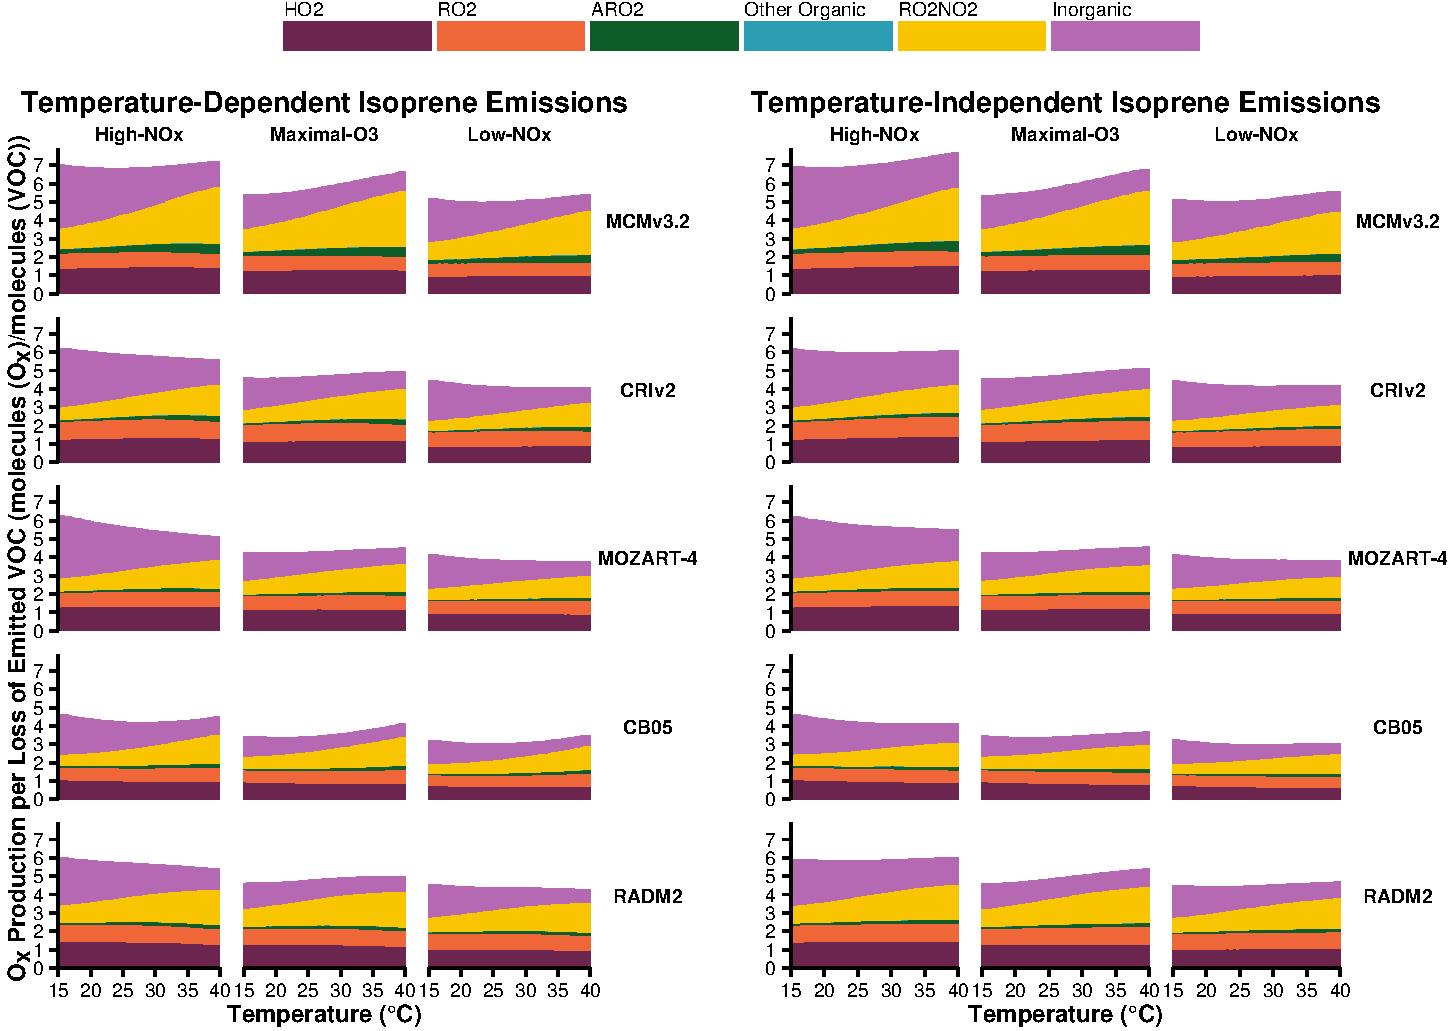
\includegraphics[width=\textwidth]{img/Ox_budgets}
\end{figure}

In order to determine which chemical processes are causing the increase in ozone with temperature (Sect.~\ref{ss:r_contours}), we analyse the \ce{O_x} production budgets in each \ce{NO_x} regime (low-\ce{NO_x}, Maximal-\ce{O3} and high-\ce{NO_x}) defined in Sect.~\ref{ss:r_contours}.
We defined the \ce{O_x} family to consist of \ce{O3}, \ce{NO2} and O, and Fig.~\ref{f:ozone_budgets} displays the total day-time \ce{O_x} production budgets normalised by the total initial oxidation rates of the emitted NMVOC for each chemical mechanism within each \ce{NO_x} regime.
The \ce{O_x} production budgets in Fig.~\ref{f:ozone_budgets} are allocated to the major sources, where `HO2', `RO2', `ARO2' represent the reactions of NO with \ce{HO2}, alkyl peroxy radicals and acyl peroxy radicals respectively.
`RO2NO2' represents the thermal decomposition of peroxy nitrates, `Inorganic' represents all inorganic contributions to the \ce{O_x} production budgets (primarily the de-excitation of \ce{O^1D} to O) and any other remaining organic reactions producing \ce{O_x} are included in the `Other Organic' category.

In Fig.~\ref{f:ozone_budgets} the number of molecules of \ce{O_x} produced per molecule of NMVOC oxidised in High-\ce{NO_x} conditions is similar when using temperature-dependent or temperature-independent isoprene emissions for each chemical mechanism; the same is also true for the Maximal-\ce{O3} and Low-\ce{NO_x} regimes.
Thus the increases in isoprene emissions in the temperature-dependent simulations are balanced by the faster oxidation rates of the emitted NMVOC.
The highest amount of \ce{O_x} is produced in the High-\ce{NO_x} regime and the lowest amount of \ce{O_x} is produced in the Low-\ce{NO_x} regime, mirroring the \ce{O3} mixing ratios in the different \ce{NO_x} regimes in Fig.\ref{f:O3-T}.
For example, when using MCMv3.2 seven molecules of \ce{O_x} are produced per molecule of NMVOC oxidation in High-\ce{NO_x} conditions, decreased to about six and five molecules of \ce{O_x} produced per molecule of NMVOC oxidised in the Maximal-\ce{O3} and Low-\ce{NO_x} regimes.
In each \ce{NO_x} regime, all the reduced chemical mechanisms produce up to two molecules of \ce{O_x} per molecule of emitted NMVOC oxidised less than the MCMv3.2.

Turning to the individual contributions to the normalised production of \ce{O_x} in Fig.~\ref{f:ozone_budgets}, peroxy nitrate (RO2NO2) decomposition and inorganic reactions show a strong (and opposing) dependence on temperature in all \ce{NO_x} regimes, each chemical mechanism and regardless of the source of isoprene emissions.
Whereas the contributions of the reaction of NO with the peroxy radicals (HO2, RO2 and ARO2 in Fig.~\ref{f:ozone_budgets}) to the normalised production budgets of \ce{O_x} do not increase strongly with temperature indicating that these processes are strongly related to the faster oxidation of the emitted NMVOC with temperature.

\subsubsection{Peroxynitrates}
We shall now turn our focus to the peroxy nitrate (RO2NO2) contribution as this category has a strongly temperature-dependent contribution to the normalised \ce{O_x} production.
Peroxy nitrates are an important reservoir species for both peroxy radicals and \ce{NO_x} that are formed from the reactions of alkyl and acyl peroxy nitrates with \ce{NO2} (Reaction \ref{r:RO2_NO2}).
\begin{rxnarray}
    && \ce{RO2 + NO2 + M} \rightleftharpoons \ce{RO2NO2 + M} \label{r:RO2_NO2}
\end{rxnarray}
The chemical bond of \ce{RO2NO2} is quite weak with thermal decomposition being the most important chemical reaction and thermal decomposition depends strongly on temperature.
At low temperatures, \ce{RO2NO2} can accumulate and be transported downwind of emissions of the sources of its precursors (NMVOC and \ce{NO_x}), after thermal decomposition the release of \ce{NO2} and peroxy radicals can promote production of \ce{O3} downwind \citep{Moxim:1996}.

Peroxy nitrates are formed from both alkyl and acyl peroxy radicals, with the acyl peroxy radicals being more thermally stable than the alkyl peroxy nitrates.
The most important alkyl peroxy nitrates are pernitric acid (\ce{HO2NO2}) and methylperoxy nitrate (\ce{CH3O2NO2}), while peroxy acetyl nitrate (PAN, \ce{CH3C(O)O2NO2}) and peroxy propionyl nitrate (PPN, \ce{C2H5C(O)O2NO2}) are important acyl peroxy nitrates.

The alkyl peroxy nitrates have a weaker \ce{RO2-NO2} bond than acyl peroxy nitrates hence alkyl peroxy nitrates have a shorter lifetime than acyl peroxy nitrates.
For example, \ce{CH3O2NO2} has a lifetime of $0.5$~seconds at $298$~K while PAN has a lifetime of $51$~minutes at $298$~K \citep{Orlando:2012}.

Each chemical mechanism used in our study represents \ce{HO2NO2} and PAN, although in many reduced chemical mechanisms PAN represents \ce{CH3C(O)O2NO2} and other acyl peroxy nitrates.
This representation of PAN in reduced chemical mechanisms can lead to overestimations of PAN levels compared to more detailed chemical mechanisms \citep{Luecken:1999}.
The near-explicit MCMv3.2 represent a diverse range of peroxy nitrates including \ce{CH3O2NO2} and about $280$~acyl peroxy nitrates.

\begin{figure}[t]%
    \centering%
    \caption{Day-time \ce{RO2NO2} production budgets normalised by the total oxidation rate of emitted VOC in the \ce{NO_x}-regimes of Fig.~\ref{f:ozone_contours}. The total budgets are allocated to the most important peroxy nitrates and all other contributions included as `Others'.}%
    \label{f:ro2no2_budgets}%
    \includegraphics[width=\textwidth]{img/RO2NO2_budgets}
\end{figure}

Figure~\ref{f:ro2no2_budgets} displays the normalised production budgets of \ce{RO2NO2} by the total loss rate of the emitted NMVOC, similar to Fig.~\ref{f:ozone_budgets} for each chemical mechanism in each \ce{NO_x} regime and when using a temperature-independent and temperature-dependent source of isoprene emissions.
The large contribution of \ce{CH3O2NO2} in MCMv3.2 is not mirrored in any reduced chemical mechanism as \ce{CH3O2NO2} is not represented in any of the reduced chemical mechanisms.
In fact the number of molecules of \ce{RO2NO2} per molecules of NMVOC oxidised in each reduced chemical mechanism is very similar to that of MCMv3.2 less the contribution of \ce{CH3O2NO2} for the separate \ce{NO_x} regimes and regardless of isoprene source.

The contribution of RO2NO2 to the normalised \ce{O_x} production in Fig.~\ref{f:ozone_budgets} is largest in the MCMv3.2 than the reduced chemical mechanisms due to the representation of \ce{CH3O2NO2} in the MCMv3.2.
If reduced chemical mechanisms represent \ce{CH3O2NO2} chemistry then this would improve the representation of the total \ce{RO2NO2} production which would have the added effect of improving the representation of \ce{O_x} production budgets.

%\subsection{Rate of Change of Ozone with Temperature} \label{ss:r_mO3-T}
%
%\begin{figure}%
%    \centering%
%    \caption{Correlation of mean ozone mixing ratio with temperature in Low-NOx, maximal-O3 and High-NOx conditions for each chemical mechanism. A linear relationship between mean ozone mixing ratios and temperature is inferred, regression statistics are found in Table~\ref{t:O3_T_stats}.}%
%    \label{f:rate_O3_T}%
%    %\includegraphics[width=\textwidth]{img/Mean_O3_T_NOx_conditions}
%\end{figure}
%
%\begin{table}%
%    \centering%
%    \caption{Regression statistics for the linear relationship between ozone mixing ratios and temperature shown in Figure~\ref{f:rate_O3_T}.}%
%    \label{t:O3_T_stats}%
%    \scalebox{.78}[.78]{{\renewcommand{\arraystretch}{1.2}
\begin{tabular}{c|c|cc|cc|cc}
	\hline\hline
    \multirow{2}{*}{\textbf{Mechanism}} & \multirow{2}{*}{\textbf{Isoprene Emissions}} & \multicolumn{2}{c|}{\textbf{Low-\chem{NO_x}}} & \multicolumn{2}{c}{\textbf{Maximal-\chem{O_3}}} & \multicolumn{2}{|c}{\textbf{High-\chem{NO_x}}} \\
    & & \textbf{Mixing} & \textbf{No Mixing} & \textbf{Mixing} & \textbf{No Mixing} & \textbf{Mixing} & \textbf{No Mixing} \\
	\hline\hline
	\multirow{2}{*}{MCMv3.2} & Temperature Independent & 0.28 & 1.01 & 0.51 & 1.36 & 0.59 & 0.96 \\ 
    & Temperature Dependent & 0.42 & 1.48 & 0.74 & 2.16 & 0.93 & 2.63 \\ 
	\hline
	\multirow{2}{*}{CRIv2} & Temperature Independent & 0.25 & 0.93 & 0.47 & 1.27 & 0.55 & 0.88 \\ 
    & Temperature Dependent & 0.40 & 1.44 & 0.71 & 2.09 & 0.90 & 2.52 \\ 
	\hline
	\multirow{2}{*}{MOZART-4} & Temperature Independent & 0.25 & 0.97 & 0.44 & 1.21 & 0.49 & 0.59 \\ 
    & Temperature Dependent & 0.38 & 1.43 & 0.65 & 1.98 & 0.81 & 2.05 \\ 
	\hline
	\multirow{2}{*}{CB05} & Temperature Independent & 0.39 & 1.30 & 0.67 & 1.72 & 0.79 & 1.45 \\ 
    & Temperature Dependent & 0.52 & 1.72 & 0.89 & 2.44 & 1.12 & 2.94 \\ 
	\hline
	\multirow{2}{*}{RADM2} & Temperature Independent & 0.37 & 1.31 & 0.61 & 1.64 & 0.70 & 1.28 \\ 
    & Temperature Dependent & 0.48 & 1.68 & 0.79 & 2.22 & 0.97 & 2.49 \\ 
	\hline\hline
\end{tabular}}}

%\end{table}
%
%Each model run was allocated the three \ce{NO_x}-conditions as described in Sect.~\ref{ss:r_budgets} and then the mean ozone mixing ratio in these \ce{NO_x} regimes were then correlated with temperature as shown in Fig.~\ref{f:rate_O3_T}.
%In literature, a linear relationship is typically reported between ozone and temperature and so the linear regression statistics are reported in Table~\ref{t:O3_T_stats}.
%
%The linear increase of ozone with temperature, m$_{\text{O3-T}}$ in Table~\ref{t:O3_T_stats}, is highest at high-NOx conditions for each chemical mechanism and for each temperature case of isoprene emissions.
%The high-NOx regime corresponds to the top regions of the contour plots in Fig.~\ref{f:ozone_contours} where increases in temperature would shift the ozone production towards the ridge of maximal ozone production, thus this increase in m$_{\text{O3-T}}$ is expected.
%Similarly, the lowest m$_{\text{O3-T}}$ are achieved in the low-NOx regime, the bottom regions of the contours in Fig.~\ref{f:ozone_contours}, where increases in temperature do not neccisarily lead to increased ozone levels.
